\documentclass[11pt]{article}
\usepackage[a4paper,margin=1in]{geometry}
\usepackage{booktabs}
\usepackage{graphicx}
\usepackage{amsmath,amssymb}
\usepackage{microtype}
\usepackage{hyperref}
\usepackage{xcolor}
\usepackage{natbib}
\usepackage{caption}
\usepackage{subcaption}
\usepackage{siunitx}
\usepackage{array}
\usepackage{longtable}
\hypersetup{colorlinks=true,linkcolor=blue,citecolor=blue,urlcolor=blue}
\graphicspath{{figures/}{images/}}

\newcommand{\pending}[1]{\textcolor{red}{[PENDING: #1]}}
\newcommand{\method}[1]{\textsc{#1}}
\newcommand{\safeinput}[1]{\IfFileExists{#1}{\input{#1}}{\textcolor{red}{[PENDING TABLE: #1]}}}

\title{ActionShap: Intervention-Grounded Evaluation of Actionable Explanations in Recommendation}
\author{Mouad Louhichi \and Redwane Nesmaoui \and Mohamed Lazaar}
\date{}

\begin{document}
\maketitle

\begin{abstract}
Recommendation explanations are commonly evaluated with deletion-based faithfulness measures, although deployed recommendation systems are used through feasible changes to user profiles, item exposure, or interaction influence. A factor can therefore be faithful under deletion while being infeasible or ineffective under an operational intervention. We introduce \textbf{ActionShap}, an intervention-grounded protocol for evaluating actionable explanations in recommendation. For each user, ActionShap defines a player set of retained historical interactions, a frozen candidate set, a declared intervention policy, and a ranking-quality utility. It measures whether an explanation ranking predicts the realized effect of feasible interventions using Attribution--Intervention Alignment, top-$k$ intervention precision, intervention regret, intervention success, and attribution stability. The protocol supports arbitrary attribution methods; Monte Carlo Shapley is included as one cooperative attribution baseline because the user-specific player set is too large for exact enumeration. The primary analysis compares deletion faithfulness with bounded feasible downweighting and evaluates joint interventions at budget two. Across five seeds and 500 users per seed, feasible-action AIA is 0.749 for Monte Carlo Shapley and 0.919 for LIME, while deletion-faithfulness alignment is 0.736 and 0.934, respectively. The corresponding actionability gaps are positive for Shapley (+0.013) and negative for LIME (−0.016), with seed-level 95\% intervals reported in Table~\ref{tab:actionability-gap}. These values are descriptive until the paired user-level inference table is generated and reported.
\end{abstract}

\textbf{Keywords:} explainable recommendation; actionability; feasible intervention; faithfulness; Shapley value; counterfactual evaluation

\section{Introduction}
Explanation methods are increasingly used to support decisions about opaque recommendation systems. Yet the dominant evaluation question is often whether a prediction changes after a feature or interaction is deleted. This is not necessarily the question faced by a system operator: an interaction may be discounted rather than removed, and a feasible action may have an effect different from an extreme deletion.

We study the resulting faithfulness--actionability gap. We ask whether an explanation identifies factors whose feasible modification produces a predictable change in ranking quality. ActionShap is an evaluation protocol rather than a new recommender architecture. It can wrap any attribution method and evaluates the method against a declared offline intervention policy.

Our contributions are: (i) a recommendation-specific protocol for intervention-grounded explanation evaluation; (ii) AIA and decision-level metrics for alignment, intervention precision, and regret; (iii) a leakage-safe temporal protocol with fixed candidate sets; and (iv) a reproducible comparison in which no attribution method is assumed to be superior in advance.

\section{Related Work}
\subsection{Recommendation explanation and faithfulness}
Prior recommendation explanations emphasize item, feature, path, or attention-based rationales. Faithfulness measures and deletion curves assess sensitivity to perturbation, but generally do not encode whether the perturbation is feasible in the deployment context.

\subsection{Counterfactual explanation and recourse}
Counterfactual explanation and algorithmic recourse explicitly reason about feasible changes \citep{wachter2017,karimi2021}. ActionShap differs by evaluating an attribution method rather than prescribing an individual recourse action, and by using ranking utility in recommendation.

\subsection{Cooperative attribution}
The Shapley value provides an axiomatic allocation of coalition value \citep{shapley1953}. SHAP and local surrogate methods make attribution practical \citep{lundberg2017,ribeiro2016}. In ActionShap, these methods are evaluation subjects; the paper does not assume that cooperative attribution is universally best.

\section{ActionShap Protocol}
\subsection{User-specific game}
For user $u$, let $P_u$ be the most recent training interactions retained under a predeclared history cap. A history-conditioned model computes a profile from the retained players at inference time. Static user embeddings are not attributed because post-hoc masking would leave their outputs unchanged.

For a coalition $S\subseteq P_u$, let
\begin{equation}
 v_u(S)=\operatorname{NDCG@K}(f_u^S,y_u),
\end{equation}
where the evaluation set is fixed once per user, contains the held-out target and a declared sample of unseen negatives, and $y_u$ is the temporal test target. This is sampled-ranking evaluation rather than retrieval; target coverage is one by construction. The empty coalition is a zero profile with a deterministic tie-break.

\subsection{Deletion and feasible intervention}
Deletion is used as a faithfulness diagnostic:
\begin{equation}
 \Delta^{\mathrm{del}}_{u,p}=v_u(P_u\setminus\{p\})-v_u(P_u).
\end{equation}
The primary feasible intervention is bounded downweighting:
\begin{equation}
 \operatorname{do}(p;\rho): w_p\leftarrow \rho w_p, \qquad \rho=0.5,
\end{equation}
with $\rho=0$ and $\rho=0.25$ as declared diagnostic and sensitivity conditions. This separation makes it possible to measure a faithfulness--actionability gap rather than reproducing leave-one-out algebraically.

\subsection{Attribution methods}
We evaluate Monte Carlo Shapley, LIME, permutation/leave-one-out attribution, and random attribution as a negative control. The same players, users, candidate sets, and intervention budgets are used for every method.

\subsection{Metrics}
The primary alignment metric is
\begin{equation}
 \operatorname{AIA}_u(g)=\operatorname{Spearman}(|\phi^g_{u,p}|,|\Delta^{\mathrm{act}}_{u,p}|),
\end{equation}
where $\Delta^{\mathrm{act}}$ is measured under the feasible intervention, not deletion. We additionally report deletion alignment, the actionability gap, top-$k$ intervention precision, intervention success, regret against a feasible oracle, and stability. A within-user permutation null calibrates AIA.

\section{Experimental Protocol}
\subsection{Data and model}
The primary benchmark is MovieLens-1M \citep{harper2016}. Interactions are temporally split with a deterministic timestamp/index tie-break. The primary model is a history-conditioned profile aggregation recommender with frozen item embeddings trained from the training split. Each user receives a fixed sampled evaluation set containing the held-out target and declared unseen negatives; the same set is reused for all coalitions. A full-catalogue subset is reserved for robustness.

\subsection{Validity and leakage controls}
We validate masking sensitivity, empty/full coalition consistency, user-locality, deterministic splits, synthetic additive-game correctness, identical-player symmetry, and AIA-null calibration. Validation and test interactions never enter the training profile or attribution player set.

\subsection{Statistical analysis}
Final method comparisons use five seeds and 500 users per seed. The primary inferential unit is the user-level paired difference; the asset notebook generates paired bootstrap intervals and within-user sign-permutation p-values for Shapley-versus-LIME and Shapley-versus-LOO comparisons. Coalition evaluations from one user are not treated as independent observations. The sampled evaluation set contains 200 items including the held-out target, giving target coverage one by construction.

\section{Results}
\subsection{Protocol validity}
The masking gate passed before the primary run. The final evaluation uses fixed sampled evaluation sets with target coverage one; the earlier retrieval-recall experiment is not used as the primary evidence. The gate figure belongs in the validity subsection or appendix, not as a headline performance result.

\subsection{Faithfulness versus actionability}
\begin{figure}[t]
  \centering
  \IfFileExists{fig02_aia_by_method.pdf}{
\includegraphics[width=.48\linewidth]{fig02_aia_by_method.pdf}}{\fbox{AIA figure pending}}
  \IfFileExists{fig02b_faithfulness_by_method.pdf}{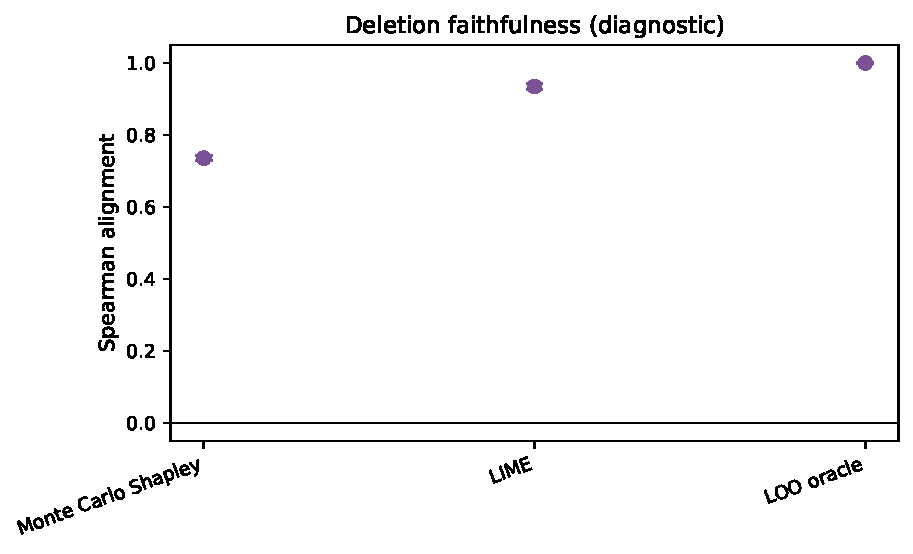
\includegraphics[width=.48\linewidth]{fig02b_faithfulness_by_method.pdf}}{\fbox{Faithfulness figure pending}}
  \caption{Intervention-grounded AIA and deletion-faithfulness alignment. Values and uncertainty must be generated from the final multi-seed result files.}
\end{figure}

The raw AIA ranking is LOO oracle, LIME, then Monte Carlo Shapley. This is not a failure of ActionShap: its purpose is to expose the difference between deletion faithfulness and feasible actionability. Shapley improves from deletion alignment to feasible-action alignment, whereas LIME decreases. The paired user-level tests and bootstrap intervals generated in `paper/tables/paired_tests.csv` determine whether this difference is statistically reliable; no universal superiority claim is made.

\subsection{Joint intervention decisions}
\begin{figure}[t]
  \centering
  \IfFileExists{fig04_joint_effect_b2.pdf}{
\includegraphics[width=.48\linewidth]{fig04_joint_effect_b2.pdf}}{\fbox{Effect figure pending}}
  \IfFileExists{fig05_joint_regret_b2.pdf}{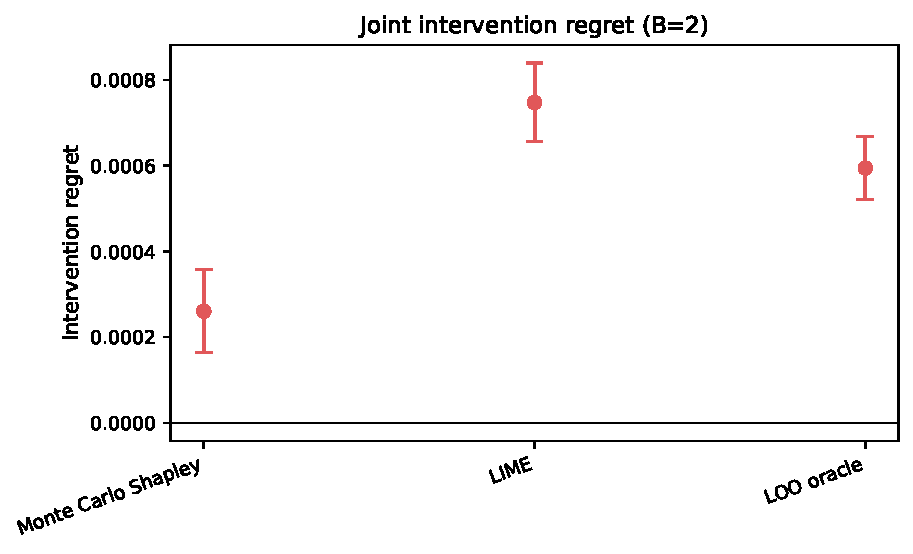
\includegraphics[width=.48\linewidth]{fig05_joint_regret_b2.pdf}}{\fbox{Regret figure pending}}
  \caption{Realized effect and regret for budget-two feasible interventions.}
\end{figure}

\safeinput{tables/protocol.tex}
\safeinput{tables/aia.tex}
\safeinput{tables/faithfulness.tex}
\safeinput{tables/actionability_gap.tex}
\safeinput{tables/joint_effect.tex}
\safeinput{tables/joint_regret.tex}
\safeinput{tables/full_catalogue_robustness.tex}
\safeinput{tables/normalized_regret.tex}
\safeinput{tables/paired_tests.tex}

\section{Robustness and Limitations}
We report sensitivity to history length, candidate size, intervention strength, Monte Carlo sample count, and random seed. Limitations include offline ranking utility, the restricted profile-intervention semantics, candidate recall, one primary recommender family, and the gap between system-executable interventions and human user recourse. ActionShap does not establish causal effects without additional causal assumptions.

\section{Conclusion}
ActionShap evaluates recommendation explanations by asking whether they predict what happens under feasible intervention. In the current five-seed, 500-user study, the feasible-intervention and deletion rankings differ systematically across the evaluated explainers, while joint intervention regret is lowest for Monte Carlo Shapley. These findings support intervention-grounded evaluation, but the final claims must follow the paired user-level tests, convergence analysis, and full-catalogue robustness results rather than raw method means alone.

\bibliographystyle{plainnat}
\bibliography{paper}
\end{document}
